\documentclass{beamer}
\usepackage{graphicx}
\usepackage{color}

\usetheme{Berlin}
\usecolortheme{beaver}
\title[A constant current applied to the HH model produces a train of action potentials.]{Step current responce of the HH Model}

\author[E.Ioannidis \& J.Hobin] {
   \texorpdfstring{
        \begin{columns}
            \column{.45\linewidth}
            \centering
            Eleftherios Ioannidis\\
            \href{mailto:elefthei@mit.edu}{elefthei@mit.edu}
            \column{.45\linewidth}
            \centering
            James Hobin\\
            \href{mailto:hobinjk@mit.edu}{hobinjk@mit.edu}
        \end{columns}
   }
   {Eleftherios Ioannidis \& James Hobin}
}


\institute{MIT EECS}
\date{\today}

% ============================================
% DOCUMENT BEGINING HERE
% ============================================

\begin{document}

% Title slide (1)
\begin{frame}
  \titlepage
\end{frame}

% slide 2
\begin{frame}{Three possible responces to a step current}
  \begin{figure}
    \centering
    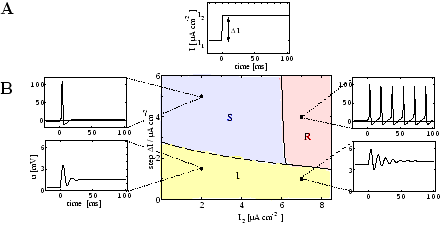
\includegraphics[width = 0.8\textwidth]{./pictures/gerstner.png}
    \caption{Phase diagram for stimulation with a step current.}
  \end{figure}
\end{frame}

% slide 0
\begin{frame}
  \begin{figure}
    \centering
    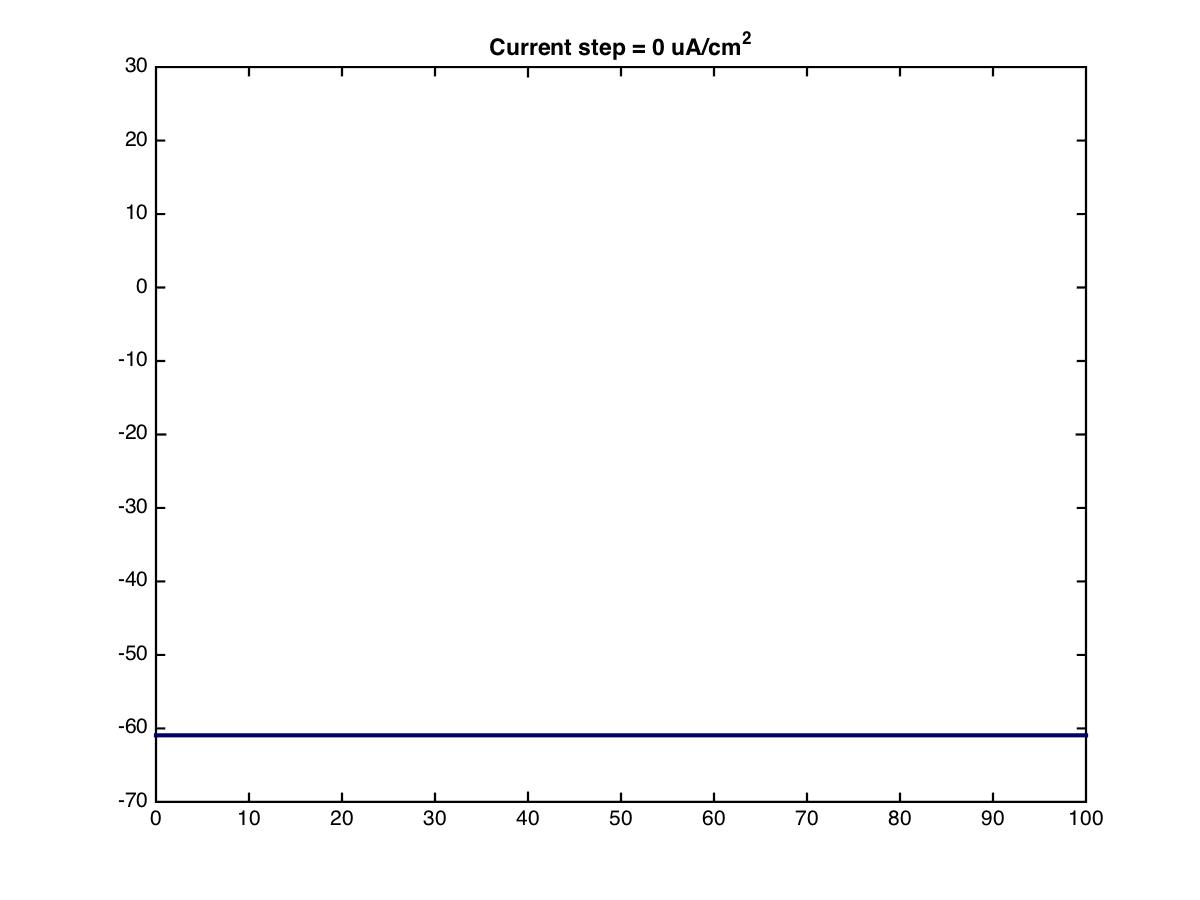
\includegraphics[width = 0.8\textwidth]{./images/current0.jpg}
    \caption{HH Models step current response starting at 0 $\mu A/cm^2$}
  \end{figure}
\end{frame}


% slide 5
\begin{frame}
  \begin{figure}
    \centering
    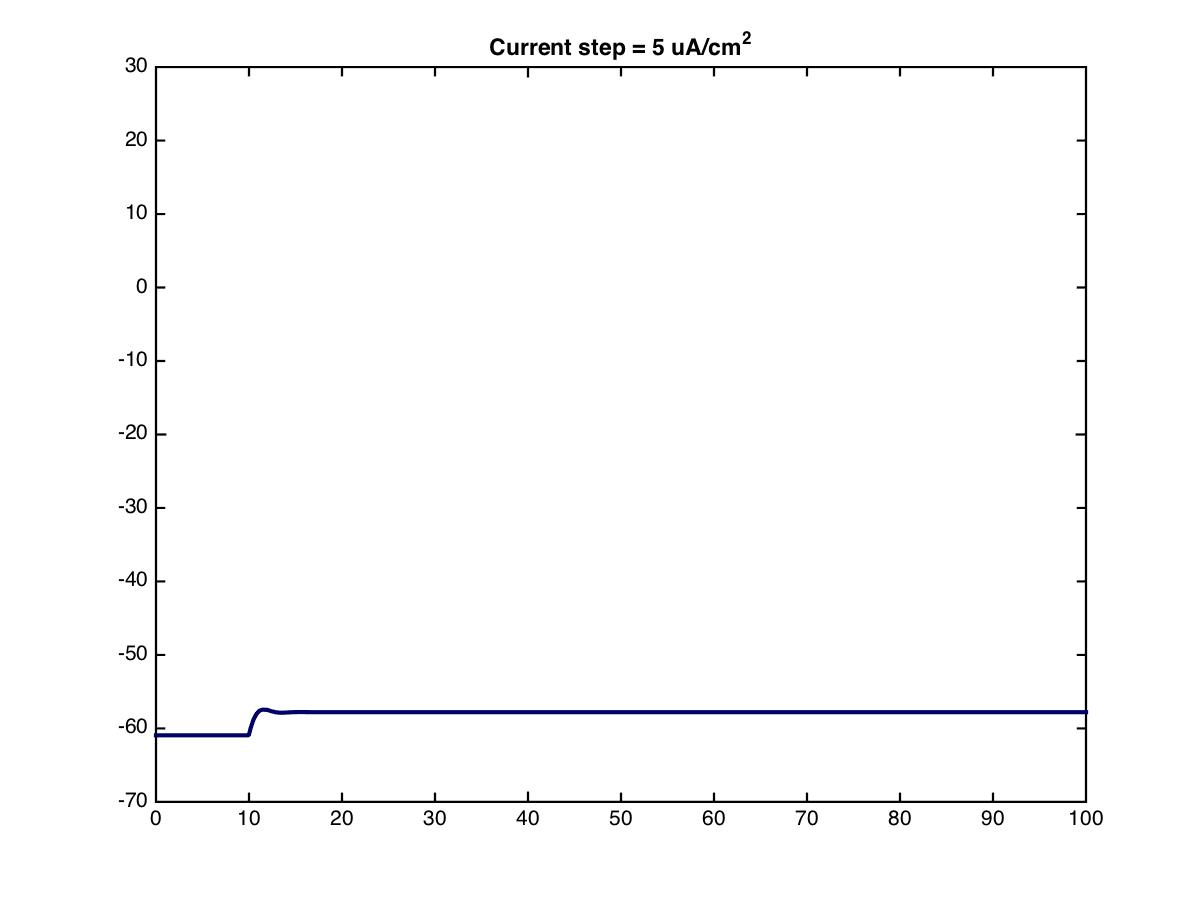
\includegraphics[width = 0.8\textwidth]{./images/current5.jpg}
    \caption{HH Models step current response starting at 0 $\mu A/cm^2$}
  \end{figure}
\end{frame}


% slide 10
\begin{frame}
  \begin{figure}
    \centering
    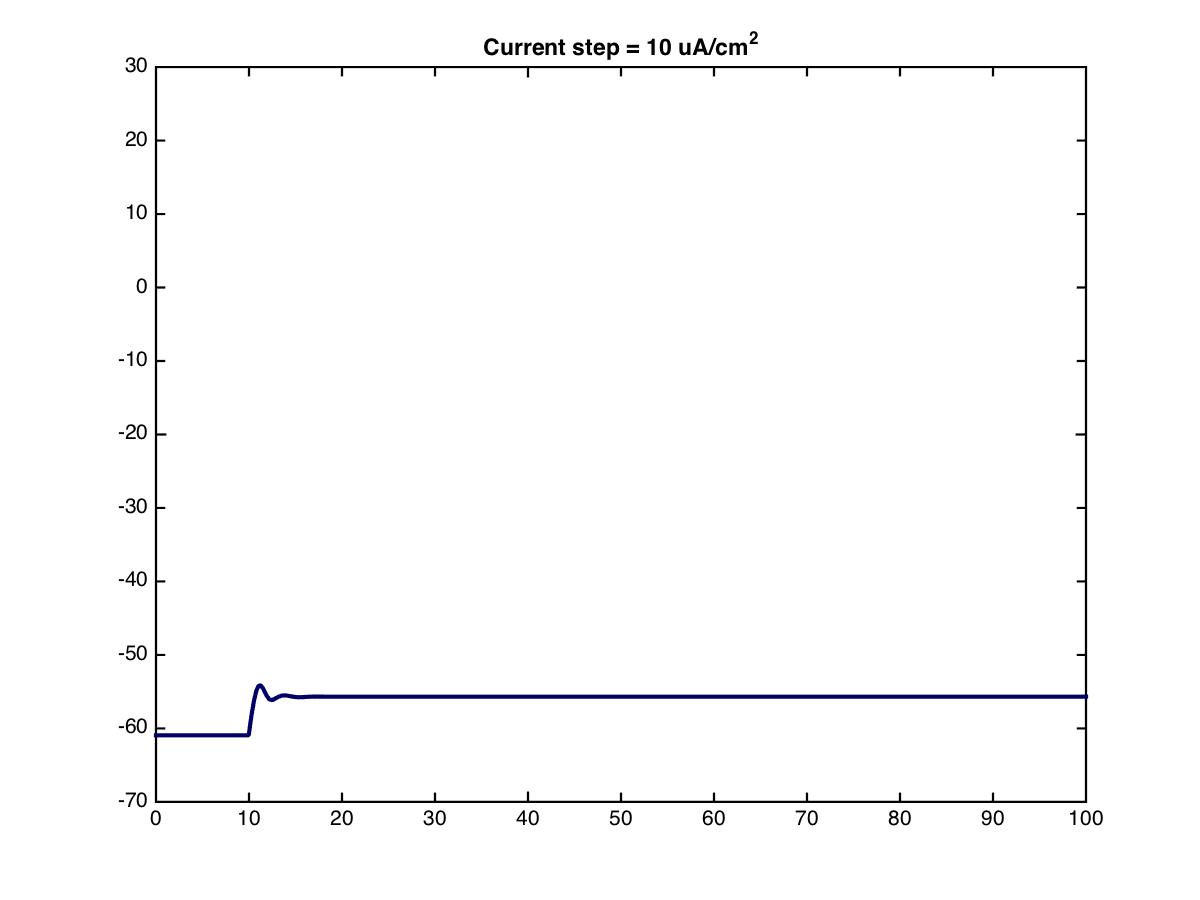
\includegraphics[width = 0.8\textwidth]{./images/current10.jpg}
    \caption{HH Models step current response starting at 0 $\mu A/cm^2$}
  \end{figure}
\end{frame}


% slide 15
\begin{frame}
  \begin{figure}
    \centering
    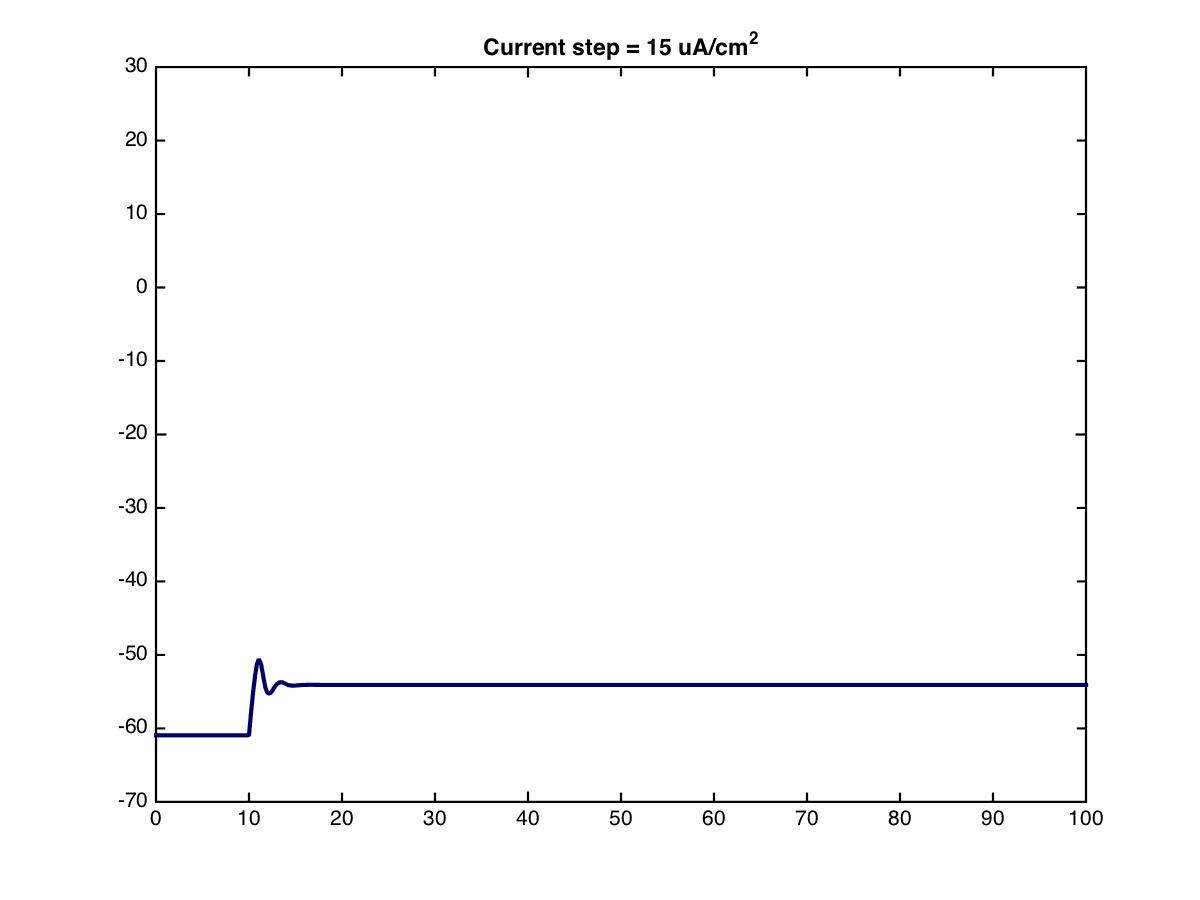
\includegraphics[width = 0.8\textwidth]{./images/current15.jpg}
    \caption{HH Models step current response starting at 0 $\mu A/cm^2$}
  \end{figure}
\end{frame}


% slide 20
\begin{frame}
  \begin{figure}
    \centering
    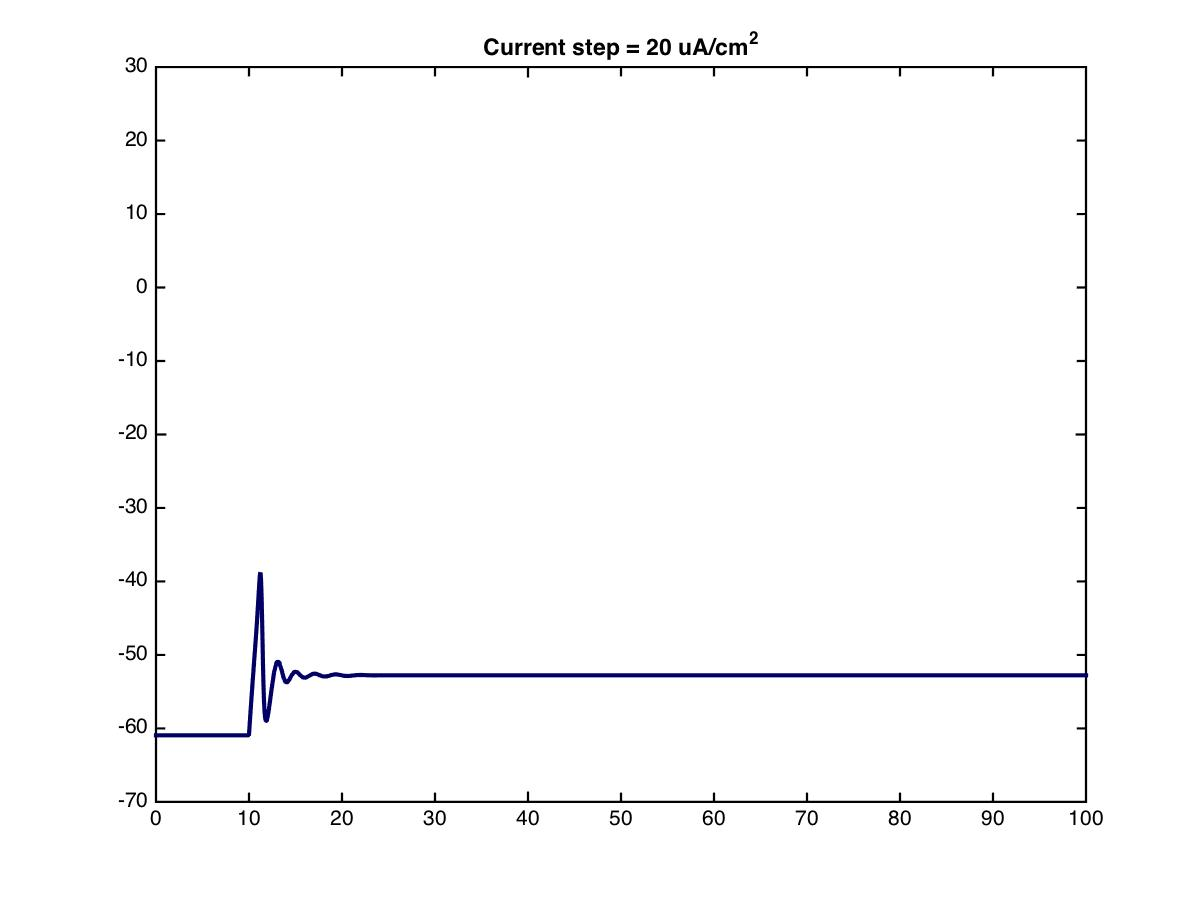
\includegraphics[width = 0.8\textwidth]{./images/current20.jpg}
    \caption{HH Models step current response starting at 0 $\mu A/cm^2$}
  \end{figure}
\end{frame}


% slide 25
\begin{frame}
  \begin{figure}
    \centering
    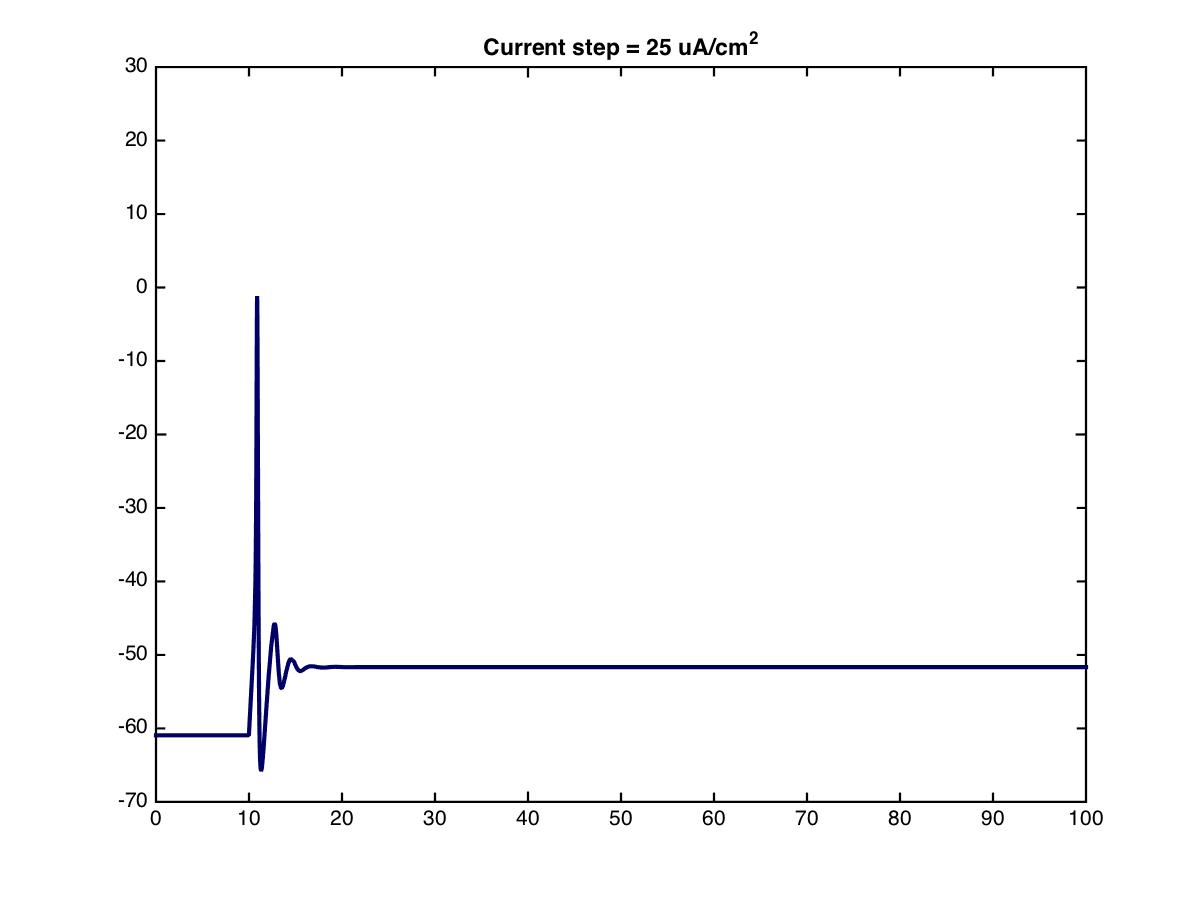
\includegraphics[width = 0.8\textwidth]{./images/current25.jpg}
    \caption{HH Models step current response starting at 0 $\mu A/cm^2$}
  \end{figure}
\end{frame}


% slide 30
\begin{frame}
  \begin{figure}
    \centering
    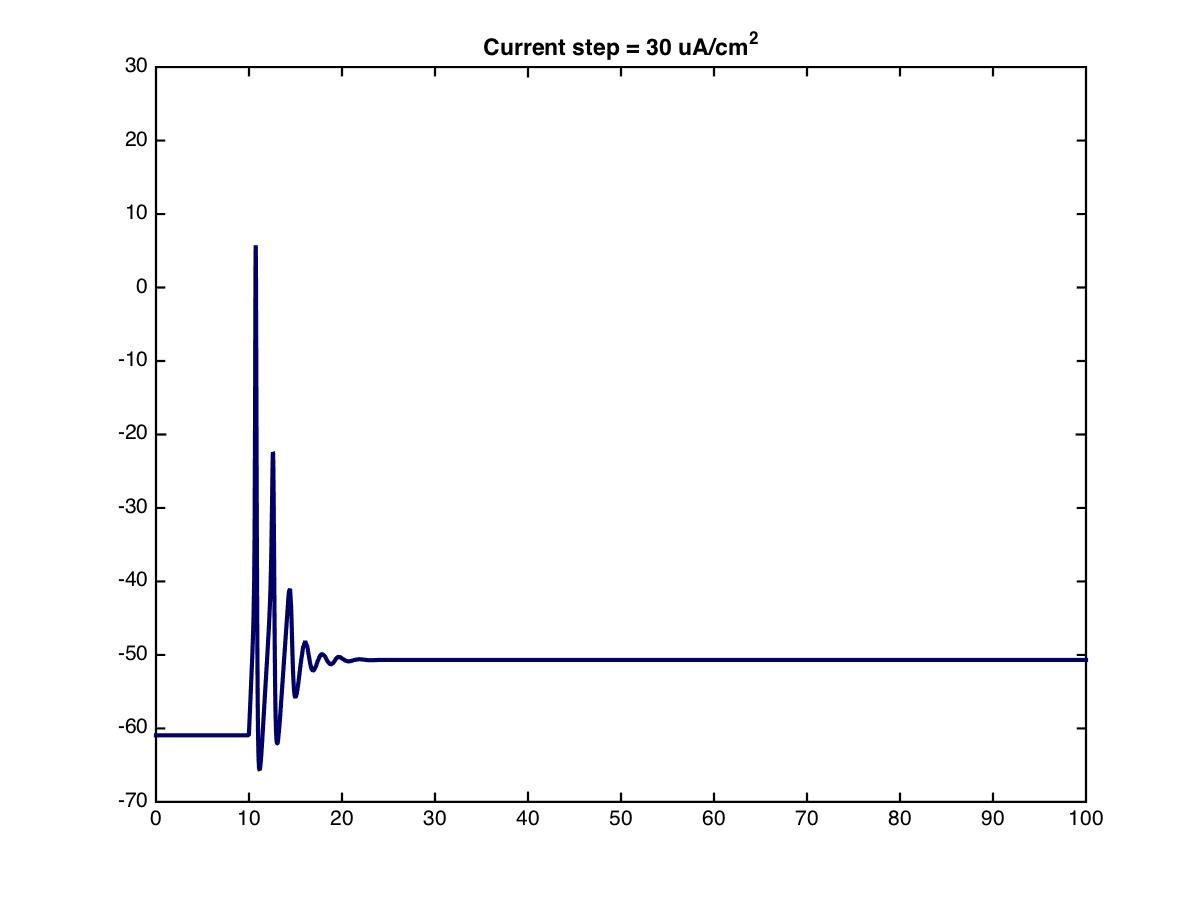
\includegraphics[width = 0.8\textwidth]{./images/current30.jpg}
    \caption{HH Models step current response starting at 0 $\mu A/cm^2$}
  \end{figure}
\end{frame}


% slide 35
\begin{frame}
  \begin{figure}
    \centering
    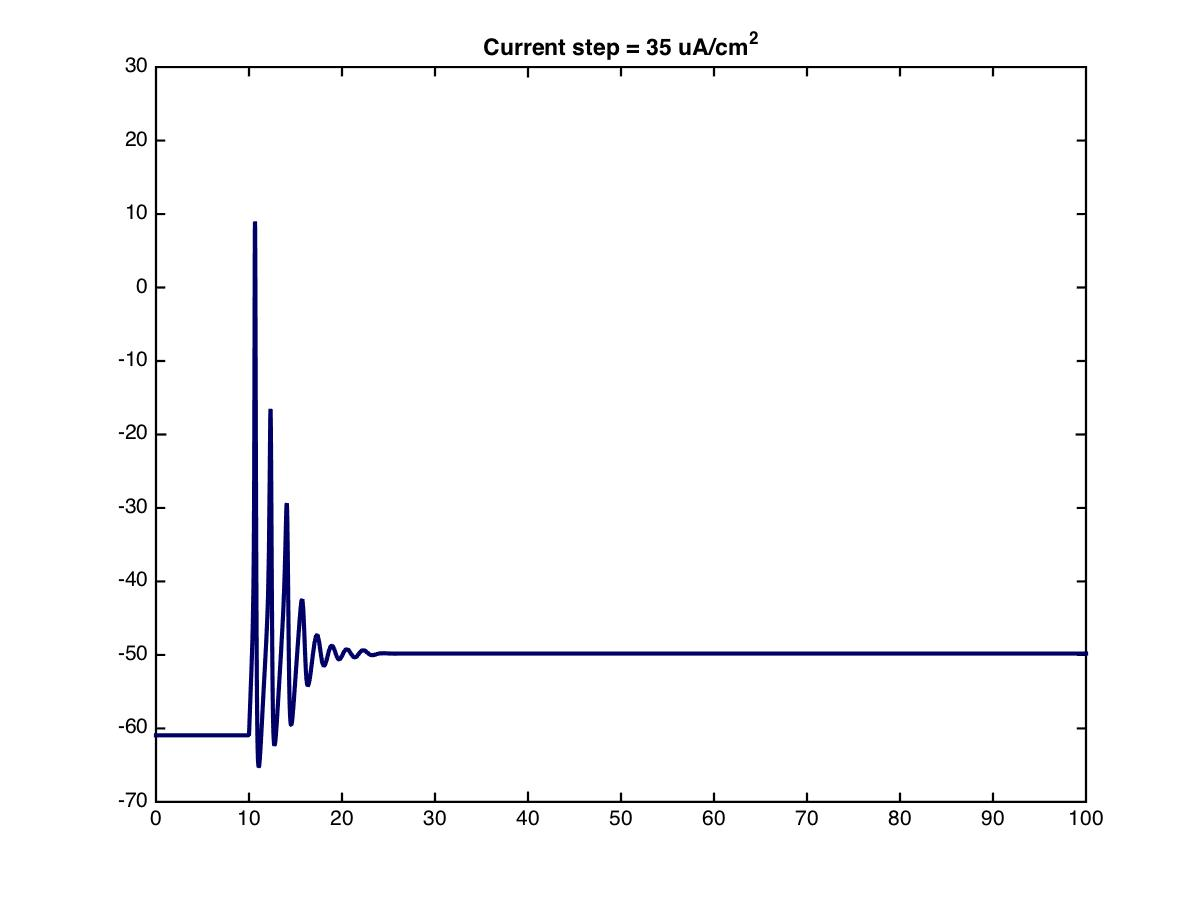
\includegraphics[width = 0.8\textwidth]{./images/current35.jpg}
    \caption{HH Models step current response starting at 0 $\mu A/cm^2$}
  \end{figure}
\end{frame}

\begin{frame}
  Finding train frequency
\end{frame}

\begin{frame}
  The three phases
\end{frame}

\begin{frame}
  Experimental design
  Precision required
\end{frame}

% slide 40
\begin{frame}
  \begin{figure}
    \centering
    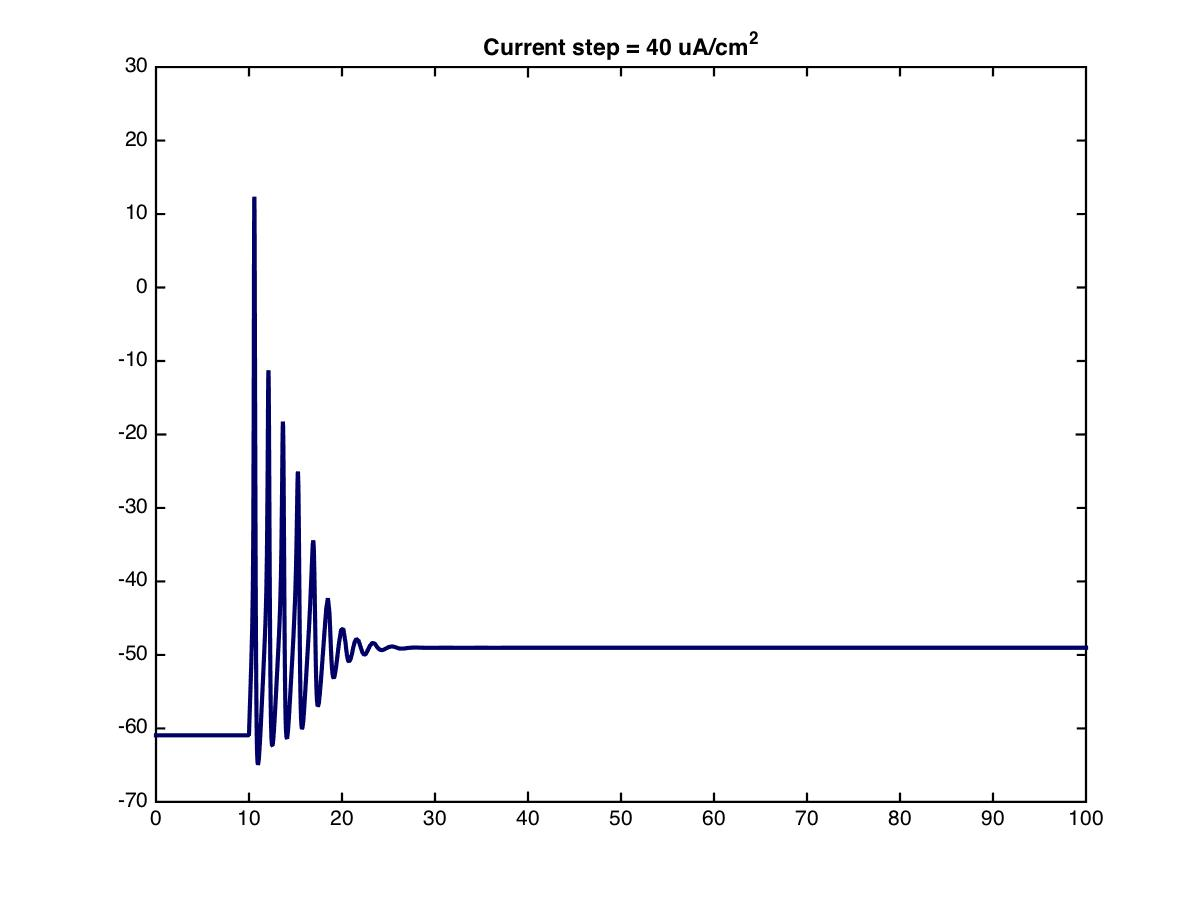
\includegraphics[width = 0.8\textwidth]{./images/current40.jpg}
    \caption{HH Models step current response starting at 0 $\mu A/cm^2$}
  \end{figure}
\end{frame}


% slide 45
\begin{frame}
  \begin{figure}
    \centering
    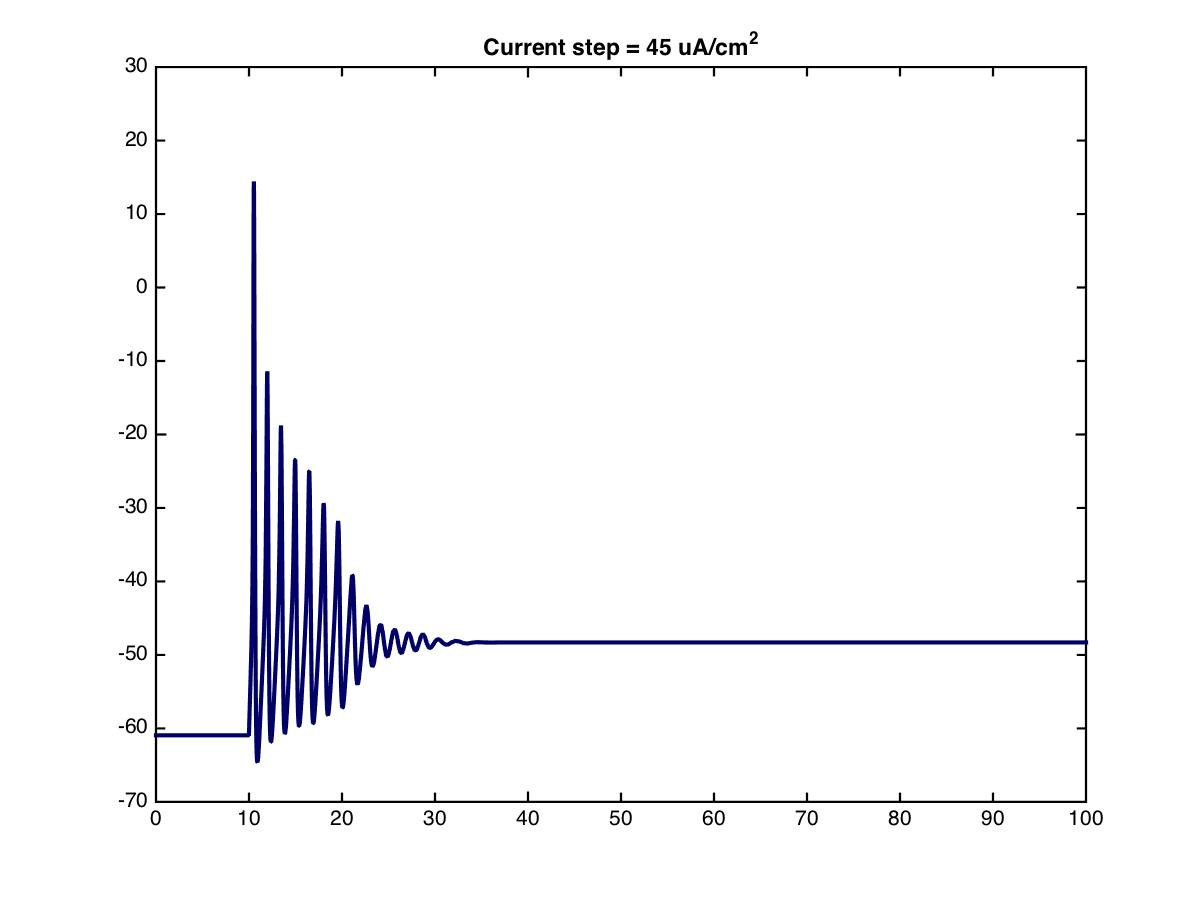
\includegraphics[width = 0.8\textwidth]{./images/current45.jpg}
    \caption{HH Models step current response starting at 0 $\mu A/cm^2$}
  \end{figure}
\end{frame}


% slide 50
\begin{frame}
  \begin{figure}
    \centering
    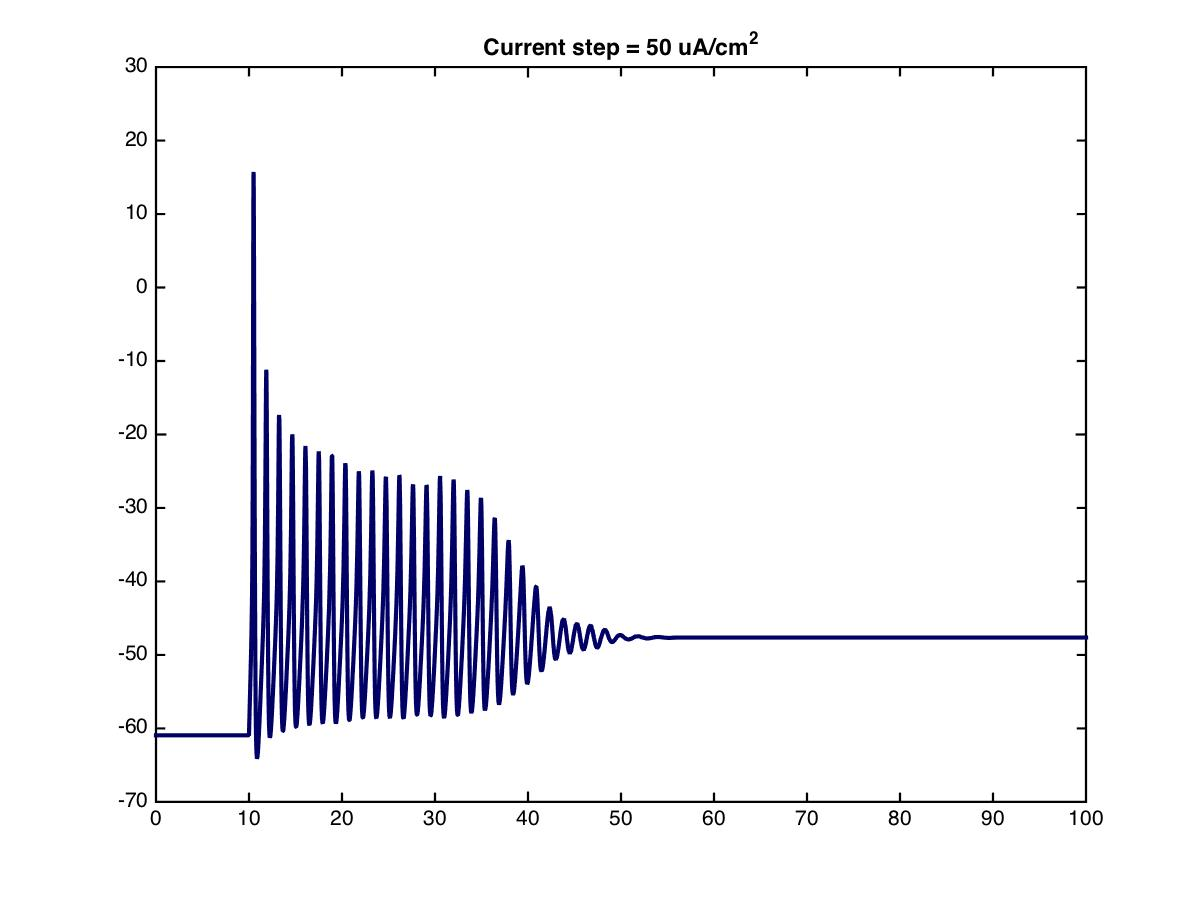
\includegraphics[width = 0.8\textwidth]{./images/current50.jpg}
    \caption{HH Models step current response starting at 0 $\mu A/cm^2$}
  \end{figure}
\end{frame}


% slide 55
\begin{frame}
  \begin{figure}
    \centering
    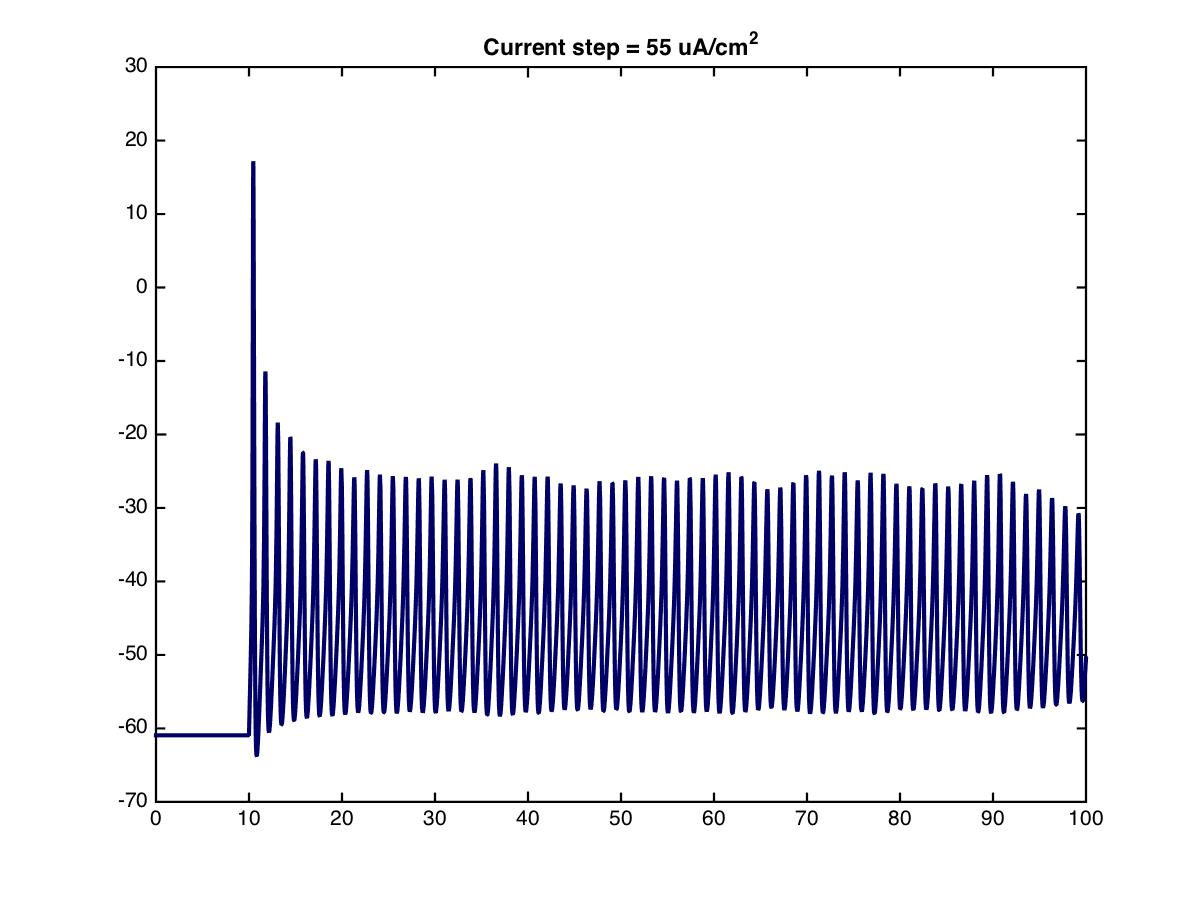
\includegraphics[width = 0.8\textwidth]{./images/current55.jpg}
    \caption{HH Models step current response starting at 0 $\mu A/cm^2$}
  \end{figure}
\end{frame}


% slide 60
\begin{frame}
  \begin{figure}
    \centering
    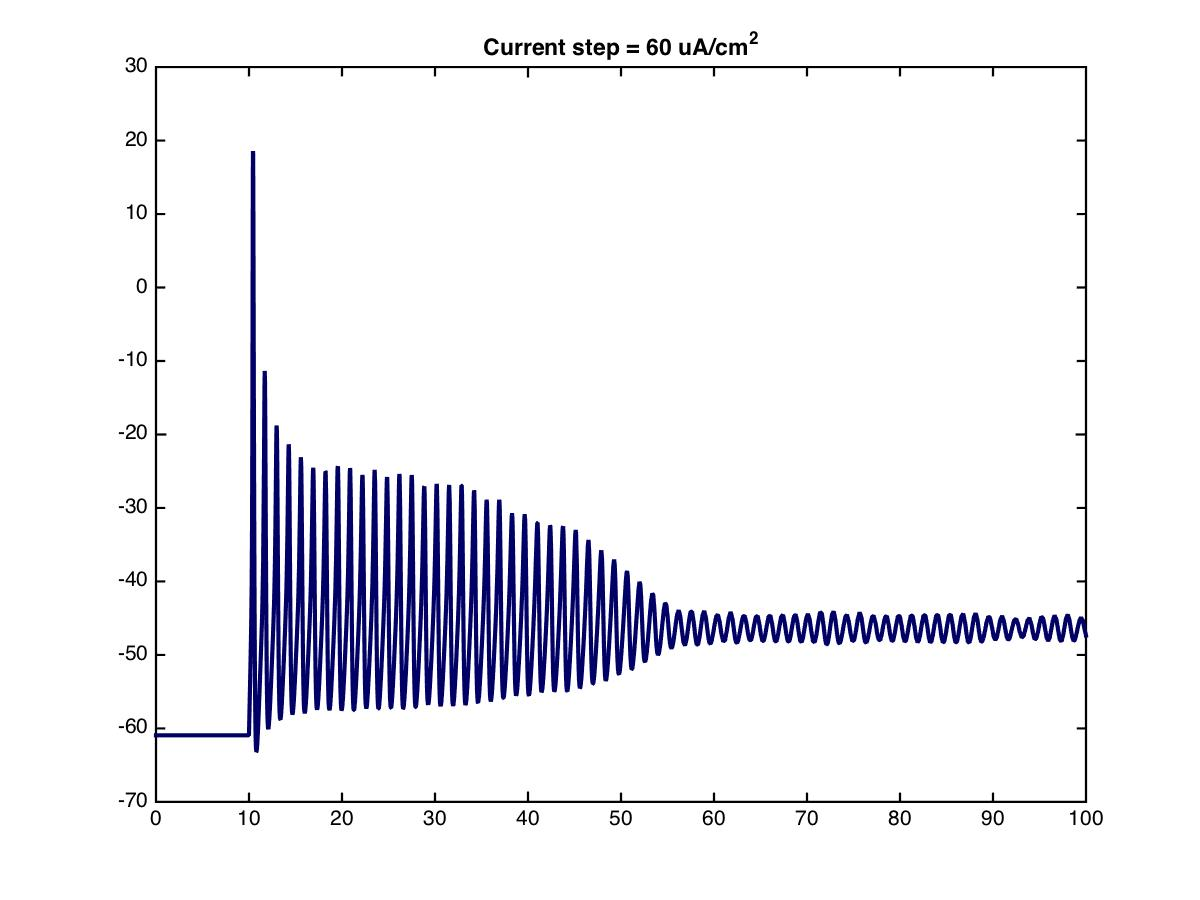
\includegraphics[width = 0.8\textwidth]{./images/current60.jpg}
    \caption{HH Models step current response starting at 0 $\mu A/cm^2$}
  \end{figure}
\end{frame}


% slide 65
\begin{frame}
  \begin{figure}
    \centering
    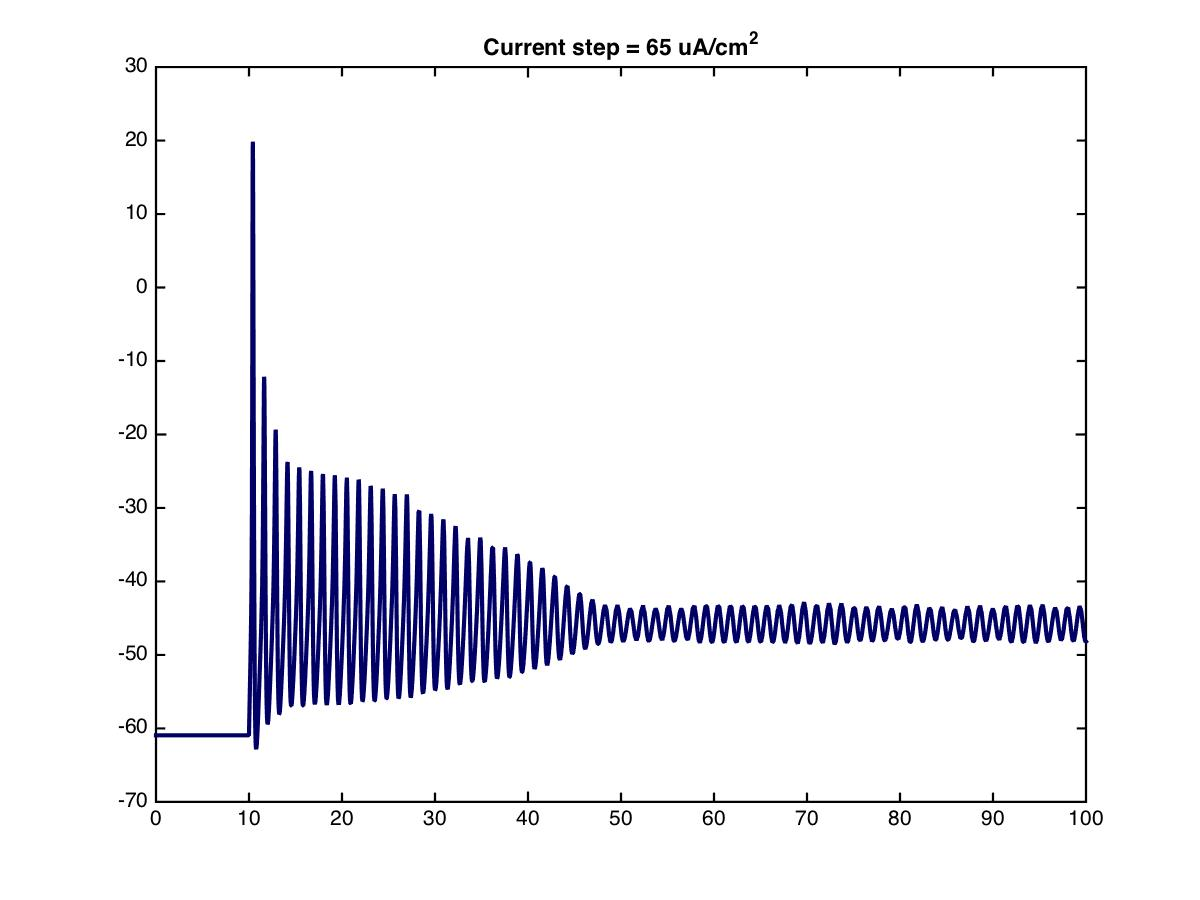
\includegraphics[width = 0.8\textwidth]{./images/current65.jpg}
    \caption{HH Models step current response starting at 0 $\mu A/cm^2$}
  \end{figure}
\end{frame}


% slide 70
\begin{frame}
  \begin{figure}
    \centering
    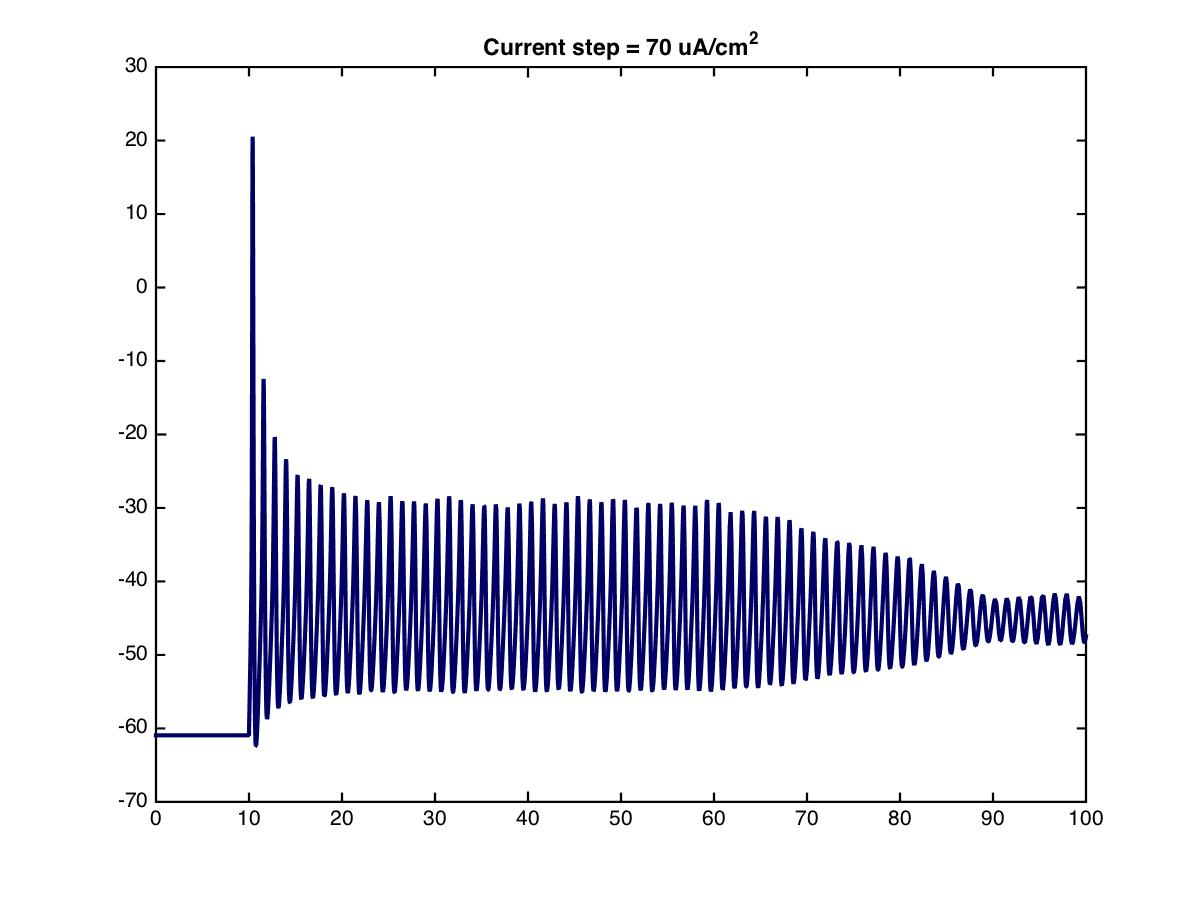
\includegraphics[width = 0.8\textwidth]{./images/current70.jpg}
    \caption{HH Models step current response starting at 0 $\mu A/cm^2$}
  \end{figure}
\end{frame}


% slide 75
\begin{frame}
  \begin{figure}
    \centering
    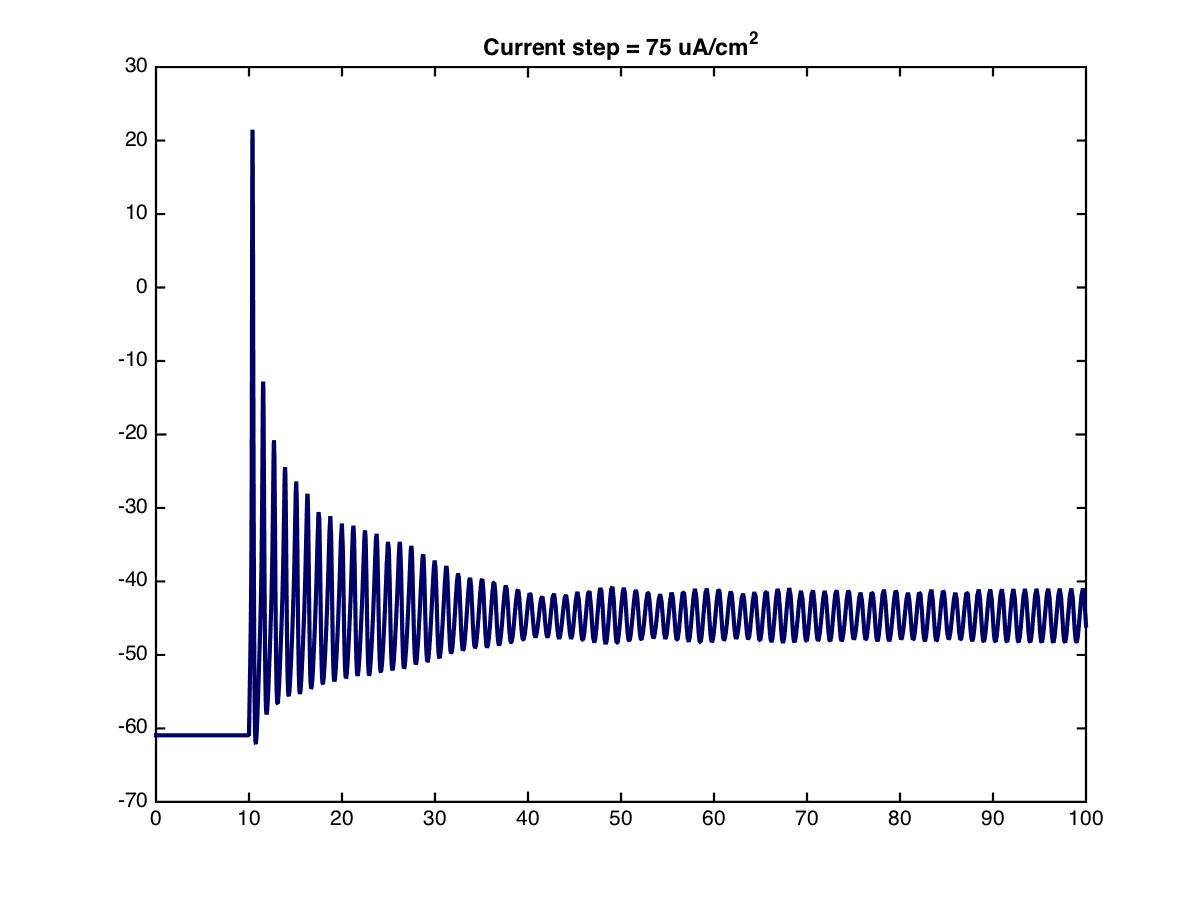
\includegraphics[width = 0.8\textwidth]{./images/current75.jpg}
    \caption{HH Models step current response starting at 0 $\mu A/cm^2$}
  \end{figure}
\end{frame}


% slide 80
\begin{frame}
  \begin{figure}
    \centering
    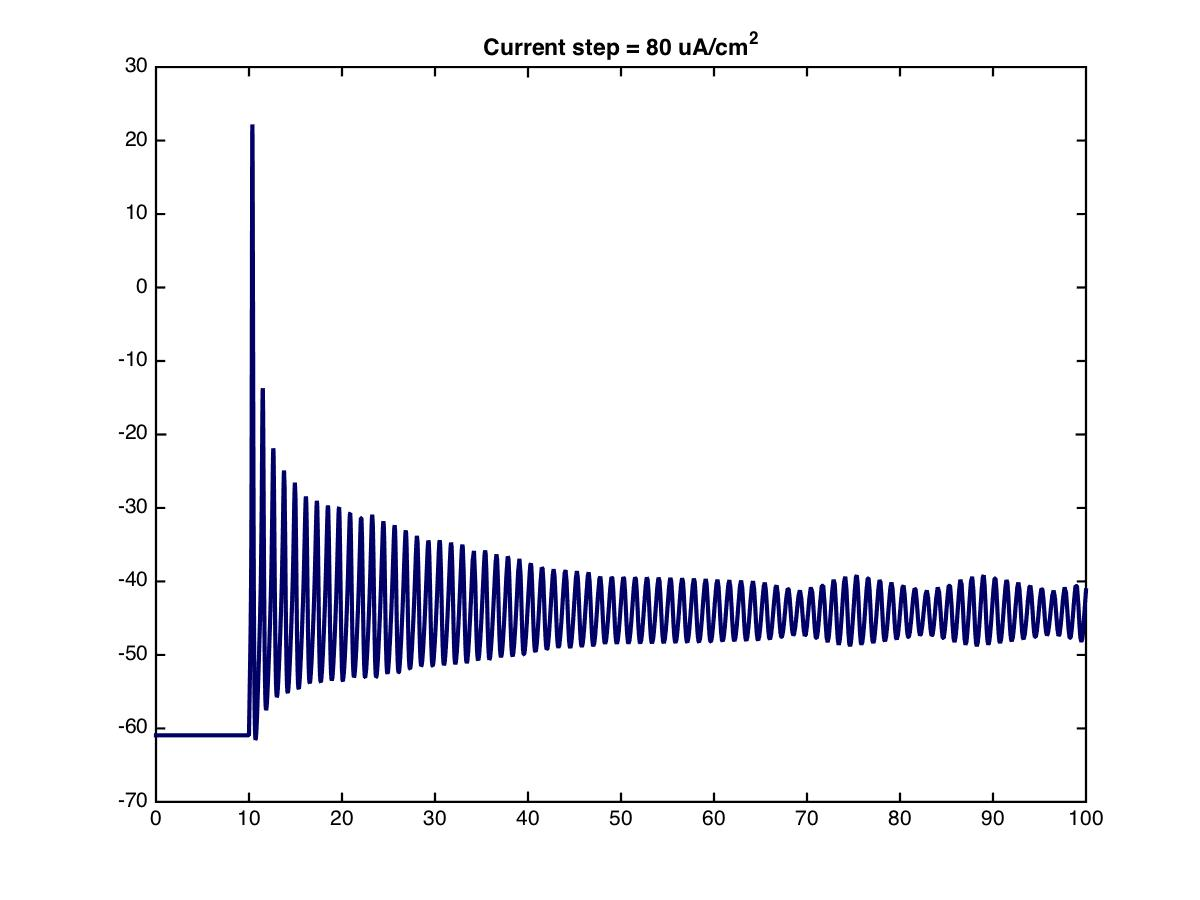
\includegraphics[width = 0.8\textwidth]{./images/current80.jpg}
    \caption{HH Models step current response starting at 0 $\mu A/cm^2$}
  \end{figure}
\end{frame}

\begin{frame}{References}
\begin{enumerate}
\item Weiss, T. F. (1995).Cellular Biophysics. Volume 1: Transport, MIT Press.
\item Weiss, T. F. (1995).Cellular Biophysics. Volume 2: Electrical Properties, MIT Press.
\item Blaustein, M.P., Kao, J.P.Y., Matteson, D.R. (2012). Cellular Physiology and Neurophysiology, 2nd edition, Elsevier-Mosby. 
\item Gerstner, Wulfram, and Werner M. Kistler. Spiking neuron models: Single neurons, populations, plasticity. Cambridge university press, 2002.
\end{enumerate}
\end{frame}
\end{document}
